%!TEX root=../GaugeCNNTheory.tex


\subsubsection*{Global rotation equivariance on $\fakebold{\Euc}_{\boldsymbol{3}} \fakebold{\backslash} \bm{\{0\}}$}
\label{sec:punctured_euclidean_3dim}

The ideas presented above can be generalized to the three-dimensional setting, i.e. to the punctured Euclidean space $\Euc_3 \backslash \{0\}$.
Globally rotation equivariant $\GM$-convolutions correspond here to $G$-structures that are invariant under $\SO3$ rotations around the origin.
While the radial dependency of such $G$-structures is left unconstrained, the demand for rotational invariance imposes a constraint on their form over spherical shells at fixed radii, which are the orbits of the action of~$\SO3$ on $\Euc_3 \backslash \{0\}$.
The fact that the sphere $S^2 = \SO3/\SO2$ is a homogeneous space of $\SO3$ with stabilizer subgroups isomorphic to $\SO2$ implies that the structure group of an $\SO3$-invariant $G$-structure can not be reduced further than $G=\SO2$; see Fig.~\ref{fig:G_structure_S2_1}.
We are therefore essentially considering spherical CNNs with an additional radial dimension.
For a review on spherical CNNs we refer the reader forward to Section~\ref{sec:instantiations_spherical}.


\citet{ramasinghe2019representation} identified this situation and designed $\SO3$-equivariant convolutions on $\Euc_3 \backslash \{0\}$.
Before coming to our classification as $\GM$-convolution, listed in  row (29) of Table~\ref{tab:network_instantiations}, we briefly review the authors' formulation and implementation.
Their implementation is based on spherical CNNs with the addition that
1) kernels extend in the radial direction and
2) are shared over shells at different radii; see Fig.~\ref{fig:G_structure_R3_no_origin} (left).
As commonly done for spherical CNNs, the angular dependency of the kernels is encoded via their Fourier spectrum on~$S^2$, that is, in terms of spherical harmonics expansion coefficients.
The sharing of these expansion coefficients implies that the shared kernels cover the same solid angle for all radii, implying that the \emph{kernels dilate in angular direction linearly with the radius}.%
\footnote{
    The dilation is here measured relative to the standard Euclidean metric of $\Euc_3 \backslash \{0\}$.
}
In the discretized implementation, the spherical shells are located at equidistant radii -- which implies that the \emph{kernels do not dilate in radial direction}.
From these insights we infer the specific $G$-structure that the model assumes below.
The kernels themselves are constrained such that they are invariant under $\SO2$ rotations around the radial axis through their center, which is often referred to as \emph{zonal kernels};
see Fig.~\ref{fig:zonal_kernel} and~\cite{esteves2018zonalSpherical}.
As proven in~\cite{esteves2018zonalSpherical} and~\cite{ramasinghe2019representation}, the convolution with such kernels is $\SO3$-equivariant.
That this is the case is intuitively clear since rotations of the spherical shells have $\SO2$ as stabilizer subgroup, w.r.t. which the zonal kernels are invariant.
As we will argue below, the model is actually $\O3$-equivariant, that is, additionally equivariant under reflections.

\begin{figure}
    \centering
    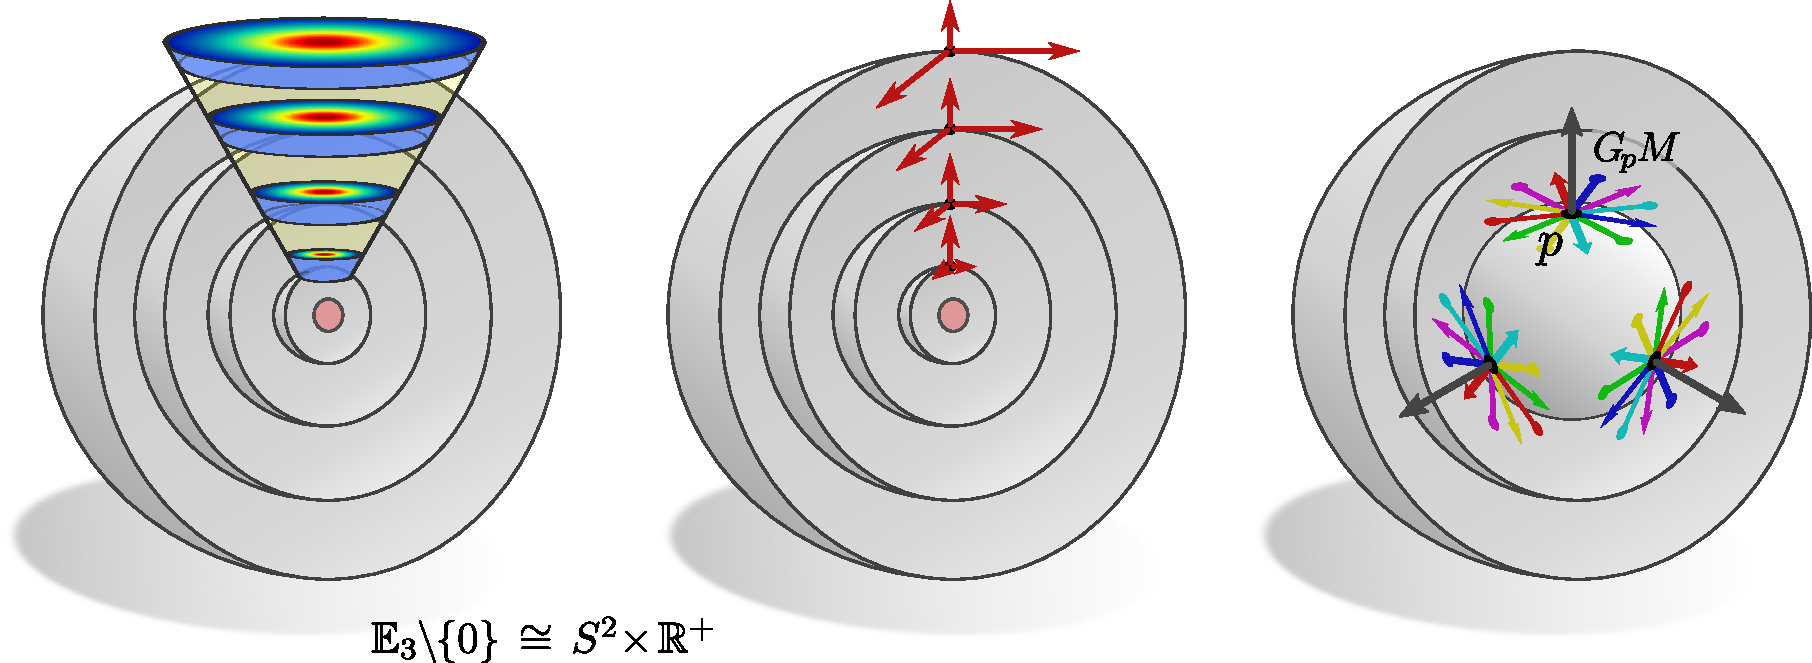
\includegraphics[width=1.\textwidth]{figures/G_structure_R3_no_origin.pdf}
    \hfill
    \caption{\small
        The $G$-structure that was implicitly assumed by~\citet{ramasinghe2019representation} can be deduced from the weight sharing scheme.
        \emph{Left:}
            Weight sharing of (isotropic) convolution kernels over $\Euc_3 \backslash \{0\} \cong S^2 \times \R^+$ as proposed in~\cite{ramasinghe2019representation}.
            The kernels are defined to cover the same solid angle, independent of the distance from the origin, such that their diameter grows linearly with this distance.
            The kernels' extent in radial direction is independent from the distance from the origin..
        \emph{Middle:}
            In our theory, kernels are shared relative to reference frames of the $G$-structure.
            To recover the proposed weight sharing scheme, $\GM$ needs to consist of frames whose axes in angular direction grow linearly with the radial distance from the origin, while the axes in radial directions need to keep their size fixed (both relative to the standard Euclidean metric).
            Such frames imply an alternative Riemannian metric on $\Euc_3 \backslash \{0\}$.
        \emph{Right:}
            As the resulting $\GM$-convolution should be $\SO3$-equivariant, the $G$-structure is required to be invariant under rotations around the origin.
            This requires (at least) an $\SO2$-structure, whose restriction to one spherical shell is shown in the right part of the figure.
            Compare this to the $\SO3$-invariant $\SO2$-structure of spherical CNNs in Fig.~\ref{fig:G_structure_S2_1}.
    }
    \label{fig:G_structure_R3_no_origin}
\end{figure}


\begin{wrapfigure}[13]{r}{0.25\textwidth}
    \vspace*{-3.ex}
    \centering
    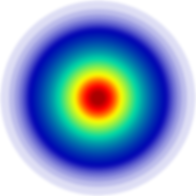
\includegraphics[width=.8\linewidth]{figures/invariant_kernel.png}%
    \caption{\small
        A \emph{zonal} (isotropic) kernel is simultaneously $\SO2$- and $\O2$-steerable;
        cf. Eqs.~\eqref{eq:Euc3_punctured_SO2_constraint} and~\eqref{eq:Euc3_punctured_O2_constraint}.
        }
    \label{fig:zonal_kernel}
\end{wrapfigure}%
To recover this model from the viewpoint of $\GM$-convolutions, we need to determine the corresponding $G$-structure on $M = \Euc_3 \backslash \{0\}$.
As stated above, the $\SO3$-equivariance of the model requires the $G$-structure to be invariant under the action of $\SO3$ but does not constrain their radial variation.
To infer this radial dependency of the $G$-structure, recall that we defined convolutional weight sharing at $p\in M$ as aligning the template kernel $K: \R^3 \to \R^{\cout\times\cin}$ relative to some (arbitrary) frame in $\GpM$ of the tangent spaces $\TpM$.
The kernel sharing considered by \citet{ramasinghe2019representation} lets us therefore draw conclusions about the implicitly considered $G$-structure.
The authors share kernels such that their area tangent to the spherical shells extends with growing distance from the origin (they cover the same solid angle at each radius) while their radial thickness remains constant.
Fig.~\ref{fig:G_structure_R3_no_origin} (left) shows this radial variation of the shared kernels while
Fig.~\ref{fig:G_structure_R3_no_origin} (middle) shows the corresponding scaling of exemplary reference frames.
Together with the required $\SO3$-invariance of the $G$-structure, this implies (at least) an $\SO2$-structure, whose restriction to one spherical shell is visualized in Fig.~\ref{fig:G_structure_R3_no_origin} (right).%
\footnote{
    The two-dimensional analog would look similar to the $G$-structure in Fig.~\ref{fig:G_structure_R2_no_origin_logpolar} but with all frame vectors in radial direction having unit norm (relative to the Euclidean metric).
}
The considered metric follows from this $G$-structure, since its frames define the relevant notion of orthonormality.
Note that this metric differs from the usual Euclidean metric.


By construction, we have rotations $\IsomGM = \SO3$ as $G$-structure preserving isometries.
$\GM$-convolutions defined by this $G$-structure, which may differ in their input and output field type, will therefore (by Theorem~\ref{thm:isom_equiv_GM_conv}) be rotation equivariant.
The specific $\GM$-convolution assumed by \citet{ramasinghe2019representation}, i.e. the assumed field types, can be deduced from the fact that the authors assume zonal kernels:
such kernels arise naturally when considering \emph{scalar fields}, i.e. trivial field representations, since the kernel constraint, Eq.~\eqref{eq:kernel_constraint}, becomes in this case 
\begin{align}\label{eq:Euc3_punctured_SO2_constraint}
    K(g\mkern1mu \mathscr{v}) = K(\mathscr{v}) \quad\ \forall\ \mathscr{v}\in\R^3,\ g\in\SO2 \,,
\end{align}
enforcing isotropic (zonal) kernels.%
\footnote{
    Kernels which map between ``scalar fields'', i.e. fields that transform according to the trivial representation of~$G$, are always $G$-invariant.
    For $G=\SO2$, this implies isotropic (zonal) kernels, while $G=\Flip$ implies the reflection invariant kernels in the upper left entry of Table~\ref{tab:reflection_steerable_kernels}.
}


As a variation of the model, one could consider the $\O2$-structure that follows from the $\SO2$-structure by adding reflected reference frames (reflecting over an arbitrary axis within the planes tangent to the spherical shells, keeping the radial frame vectors still pointing outwards).%
\footnote{
    This $\O2$-structure is the counterpart of the $\O1 = \Flip$-structure in Fig.~\ref{fig:G_structure_R2_no_origin_O2} for $d=3$ instead of $d=2$.
}
In this case one has $G$-structure preserving isometries $\IsomGM = \O3$ that consist of global rotations and reflections around the origin, and therefore $\O3$-equivariant $\GM$-convolutions.
An interesting special case in the current context is that of $\GM$-convolutions that map between scalar fields, for which the kernel constraint reads
\begin{align}\label{eq:Euc3_punctured_O2_constraint}
    K(g\mkern1mu \mathscr{v}) = K(\mathscr{v}) \quad\ \forall\ \ \mathscr{v}\in\R^3,\ g\in\O2 \,.
\end{align}
This seems like a stronger constraint than that in Eq.~\eqref{eq:Euc3_punctured_SO2_constraint} above:
instead of only demanding kernels to be rotationally invariant, it requires them additionally to be invariant under reflections.
However, since rotation invariant kernels are already invariant under reflections, this leads again to zonal kernels, and therefore exactly the same kernel space as for~$\SO2$.%
\footnote{
    More formally, we are searching for kernels that satisfy $K(g\mkern1mu \mathscr{v}) = K(\mathscr{v})\ \ \forall g\in G$, that is, which are invariant on the \emph{orbits} $G.\mathscr{v} = \{g\mkern1mu \mathscr{v} \,|\, g\in G\} \in G \backslash \R^d$ of points $\mathscr{v}$ in $\R^d$.
    As the orbits $\O2.\mathscr{v} = \SO2.\mathscr{v}$ agree for any $\mathscr{v}\in\R^3$, the resulting kernel spaces are the same.
}
This implies that the model by~\citet{ramasinghe2019representation} is actually not only $\SO3$-equivariant, as claimed by the authors, but more generally $\O3$-equivariant, which justifies our classification in row (29) of Table~\ref{tab:network_instantiations},
Note that this is a special case that applies only for scalar fields -- the spaces of $\SO2$- and $\O2$-steerable kernels differ for general group representations.


How does the model by~\citet{ramasinghe2019representation} relate to that of~\citet{esteves2017polar}, which relies on the $G$-structure shown in Fig.~\ref{fig:G_structure_R2_no_origin_logpolar}?
A key difference between the two approaches is that the $G$-structure in Fig.~\ref{fig:G_structure_R2_no_origin_logpolar} consists of frames whose outward pointing axes grow with the radial distance from the origin, which is not the case for the $G$-structure in Fig.~\ref{fig:G_structure_R3_no_origin}.
If we modify the latter to consist of frames whose radial axes grow linearly with the frames' distance from the origin, one would have $\IsomGM = \SO3 \!\times \Scale$ (instead of $\IsomGM = \SO3$).
The corresponding $\GM$-convolution would therefore additionally be scale equivariant.
In an implementation, this could easily be realized by spacing the discrete spherical shells considered by~\citet{ramasinghe2019representation} exponentially instead of uniformly (corresponding to a uniform spacing of the logarithmized radius).


Lastly, we briefly discuss the convolution by~\citet{boomsma2017spherical} that is listed in row (30) of Table~\ref{tab:network_instantiations}.
It~relies on a radial projection of the signal on spherical shells to a circumscribing cube.
To define a convolution on the cube, the authors cut it open at some of its edges and flatten it out; see Fig.~2 in their work.
Subsequently, they perform a conventional two-dimensional convolution on the flattened cube faces.
Extending this operation with a third, radial dimension, defines a convolution on $\Euc_3 \backslash \{0\}$.
As the radial shells are in the discretized implementation again spaced equidistantly, this operation corresponds to a $\GM$-convolution on an $\{e\}$-structure that varies radially as shown in Fig.~\ref{fig:G_structure_R3_no_origin}.
The projection from the spherical shells to the cube implies a distortion of the frames on each of the cubes faces, and thus to a distortion of the metric on the spherical shells.
The $\{e\}$-structure is discontinuous at most of the cuts and does therefore not allow the convolution to preserve the continuity of feature fields.
Since $S^2$ is not parallelizable, this issue can not be resolved without assuming a non-trivial structure group~$G$.
The $\{e\}$-structure as a whole is not preserved by any isometries, implying that the model's global equivariance group $\IsomeM = \{e\}$ is trivial.
However, as the restriction of the $\{e\}$-structure to the four ``vertical'' faces of the cube is invariant under rotations by multiples of $\pi/2$, the model is in practice partially equivariant w.r.t. global $\C4$-rotations around the vertical axis.
For datasets whose samples are centered around the origin $\{0\}$ and are rotationally symmetric in distribution, this property is empirically shown to lead to an improved performance in comparison to conventional convolutions on $\Euc_3$.
The authors are furthermore investigating the effect of different weight sharing schemes over the radial dimension, finding that full weight sharing works best in practice. 
